\documentclass[12pt,a4paper]{article}

\usepackage[utf8]{inputenc}
\usepackage[T1]{fontenc}
\usepackage[spanish, es-nodecimaldot]{babel}
\usepackage{geometry}
\usepackage{graphicx}
\usepackage{float}
\usepackage{booktabs}
\usepackage{array}
\usepackage{xcolor}
\usepackage{amsmath}
\usepackage{listings}
\usepackage{hyperref}
\usepackage{fancyhdr}
\usepackage{titlesec}

\geometry{
    left=1in,
    right=1in,
    top=1in,
    bottom=1in
}

\pagestyle{fancy}
\fancyhf{}
\lhead{Práctica 2: OSPF}
\rhead{Interacción de redes}
\cfoot{\thepage}

% Configuración de código
\definecolor{codegray}{gray}{0.95}

\lstdefinestyle{cisco}{
    backgroundcolor=\color{codegray},
    basicstyle=\ttfamily\small,
    frame=single,
    breaklines=true,
    columns=fullflexible,
    keepspaces=true,
    showstringspaces=false
}

\hypersetup{
    colorlinks=true,
    linkcolor=black,
    urlcolor=blue,
    citecolor=black
}

\title{
Práctica 2: OSPF\\[0.5em]
\large Interacción de redes
}

\author{
Jorge Alberto Suarez Saldana\\
\small Matrícula: 355992\\
\small Profesor: Raymundo Antonio González Grimaldo
}

\date{\today}

\begin{document}

\maketitle

\section{Introducción}

El protocolo Open Shortest Path First (OSPF) es un protocolo de
enrutamiento dinámico de estado de enlace utilizado para determinar las
rutas más adecuadas dentro de un sistema autónomo. A diferencia de los
protocolos basados en distancia, OSPF construye una representación de la
topología de la red mediante el intercambio de información entre
routers vecinos y utiliza el algoritmo Shortest Path First para
calcular las rutas.

En esta práctica se configuró el protocolo OSPF en una topología
compuesta por tres routers interconectados mediante enlaces seriales y
tres redes LAN. Además de activar el proceso OSPF, se utilizaron
diferentes métodos para asociar las interfaces al protocolo: comandos
\texttt{network} con máscaras comodín, comandos \texttt{network} con
máscara cuádruple cero y configuración directa mediante
\texttt{ip ospf} en las interfaces.

Finalmente, se configuraron interfaces pasivas para evitar el envío
innecesario de mensajes OSPF hacia las redes LAN y se verificó el
funcionamiento del protocolo mediante diferentes comandos
\texttt{show} y pruebas de conectividad.

% --------------------------------------------------
% OBJETIVOS
% --------------------------------------------------
\section{Objetivos}

\begin{itemize}
    \item Configurar el proceso de enrutamiento OSPF en tres routers.
    \item Establecer identificadores de router explícitos.
    \item Configurar OSPF utilizando instrucciones \texttt{network} y
    máscaras comodín.
    \item Configurar OSPF utilizando direcciones IP de interfaces y la
    máscara comodín \texttt{0.0.0.0}.
    \item Activar OSPF directamente sobre las interfaces de un router.
    \item Configurar interfaces LAN como interfaces pasivas.
    \item Verificar la formación de adyacencias entre routers.
    \item Comprobar que las rutas remotas fueron aprendidas mediante
    OSPF.
\end{itemize}

% --------------------------------------------------
% TOPOLOGÍA Y DIRECCIONAMIENTO
% --------------------------------------------------
\section{Topología y direccionamiento}

La topología utilizada está formada por tres routers: R1, R2 y R3.
Cada router posee una interfaz conectada a una red LAN y dos
interfaces seriales que permiten establecer comunicación con los otros
routers.

La asignación de direcciones utilizada fue la siguiente.

\begin{table}[H]
\centering
\caption{Tabla de asignación de direcciones}
\begin{tabular}{llll}
\toprule
\textbf{Dispositivo} & \textbf{Interfaz} & \textbf{Dirección IP} &
\textbf{Máscara} \\
\midrule
R1 & G0/0/0 & 192.168.10.1 & /24 \\
R1 & S0/1/0 & 10.1.1.1 & /30 \\
R1 & S0/1/1 & 10.1.1.5 & /30 \\
R2 & G0/0/0 & 192.168.20.1 & /24 \\
R2 & S0/1/0 & 10.1.1.2 & /30 \\
R2 & S0/1/1 & 10.1.1.9 & /30 \\
R3 & G0/0/0 & 192.168.30.1 & /24 \\
R3 & S0/1/0 & 10.1.1.10 & /30 \\
R3 & S0/1/1 & 10.1.1.6 & /30 \\
PC1 & NIC & 192.168.10.10 & /24 \\
PC2 & NIC & 192.168.20.10 & /24 \\
PC3 & NIC & 192.168.30.10 & /24 \\
\bottomrule
\end{tabular}
\end{table}

A partir de las direcciones anteriores se identificaron las siguientes
redes:

\begin{table}[H]
\centering
\caption{Redes utilizadas en la topología}
\begin{tabular}{lll}
\toprule
\textbf{Red} & \textbf{Prefijo} & \textbf{Máscara comodín} \\
\midrule
192.168.10.0 & /24 & 0.0.0.255 \\
192.168.20.0 & /24 & 0.0.0.255 \\
192.168.30.0 & /24 & 0.0.0.255 \\
10.1.1.0 & /30 & 0.0.0.3 \\
10.1.1.4 & /30 & 0.0.0.3 \\
10.1.1.8 & /30 & 0.0.0.3 \\
\bottomrule
\end{tabular}
\end{table}

% --------------------------------------------------
% PARTE 1
% --------------------------------------------------
\section{Parte 1: Configuración de los identificadores de router}

El primer paso consistió en iniciar el proceso OSPF con el identificador
de proceso 10 en cada uno de los routers. Posteriormente se estableció
manualmente el Router ID de cada dispositivo mediante el comando
\texttt{router-id}.

En R1 se utilizó:

\begin{lstlisting}[style=cisco]
enable
configure terminal
router ospf 10
router-id 1.1.1.1
end
\end{lstlisting}

En R2:

\begin{lstlisting}[style=cisco]
enable
configure terminal
router ospf 10
router-id 2.2.2.2
end
\end{lstlisting}

Finalmente, en R3:

\begin{lstlisting}[style=cisco]
enable
configure terminal
router ospf 10
router-id 3.3.3.3
end
\end{lstlisting}

De esta manera, los identificadores quedaron establecidos de forma
explícita y no dependieron de la selección automática de una dirección
IP por parte de OSPF.

\begin{table}[H]
\centering
\caption{Identificadores OSPF configurados}
\begin{tabular}{cc}
\toprule
\textbf{Router} & \textbf{Router ID} \\
\midrule
R1 & 1.1.1.1 \\
R2 & 2.2.2.2 \\
R3 & 3.3.3.3 \\
\bottomrule
\end{tabular}
\end{table}

% --------------------------------------------------
% PARTE 2
% --------------------------------------------------
\section{Parte 2: Configuración de redes para OSPF}

\subsection{Paso 1: R1 mediante instrucciones de red y máscaras comodín}

En R1 se configuró OSPF utilizando instrucciones \texttt{network}.
Para determinar las máscaras comodín fue necesario realizar la
resta entre \texttt{255.255.255.255} y la máscara de subred
correspondiente.

Para una red /24:

\[
255.255.255.255 - 255.255.255.0
= 0.0.0.255
\]

Por lo tanto, la máscara comodín correspondiente a /24 es
\texttt{0.0.0.255}.

Para una red /30:

\[
255.255.255.255 - 255.255.255.252
= 0.0.0.3
\]

Por lo tanto, la máscara comodín correspondiente a /30 es
\texttt{0.0.0.3}.

R1 posee tres redes directamente conectadas, por lo que fueron
necesarias tres instrucciones \texttt{network}:

\begin{lstlisting}[style=cisco]
enable
configure terminal
router ospf 10

network 192.168.10.0 0.0.0.255 area 0
network 10.1.1.0 0.0.0.3 area 0
network 10.1.1.4 0.0.0.3 area 0

end
\end{lstlisting}

La configuración permite que OSPF se active en las tres interfaces de
R1 correspondientes a sus redes conectadas.

\subsection{Paso 2: R2 mediante direcciones de interfaz y máscara
cuádruple cero}

En R2 se utilizó una segunda forma de activar OSPF. En lugar de
especificar las direcciones de red, se utilizaron directamente las
direcciones IP asignadas a las interfaces junto con la máscara
comodín \texttt{0.0.0.0}.

La configuración fue:

\begin{lstlisting}[style=cisco]
enable
configure terminal
router ospf 10

network 192.168.20.1 0.0.0.0 area 0
network 10.1.1.2 0.0.0.0 area 0
network 10.1.1.9 0.0.0.0 area 0

end
\end{lstlisting}

La máscara \texttt{0.0.0.0} hace que la coincidencia sea exacta.
Por ejemplo, la instrucción

\begin{lstlisting}[style=cisco]
network 10.1.1.2 0.0.0.0 area 0
\end{lstlisting}

hace que OSPF se active específicamente sobre la interfaz que posee la
dirección IP \texttt{10.1.1.2}.

\subsection{Paso 3: R3 mediante configuración directa de interfaces}

En R3 se utilizó una tercera técnica: activar OSPF directamente desde
la configuración de cada interfaz mediante el comando
\texttt{ip ospf}.

Primero se inició el proceso OSPF y se configuró el Router ID:

\begin{lstlisting}[style=cisco]
enable
configure terminal
router ospf 10
router-id 3.3.3.3
exit
\end{lstlisting}

Posteriormente se activó OSPF en las tres interfaces:

\begin{lstlisting}[style=cisco]
interface g0/0/0
ip ospf 10 area 0
exit

interface s0/1/0
ip ospf 10 area 0
exit

interface s0/1/1
ip ospf 10 area 0
exit

end
\end{lstlisting}

Las tres interfaces de R3 debían participar en OSPF, debido a que
G0/0/0 conecta la LAN de R3 y las dos interfaces seriales conectan al
router con R1 y R2.

% --------------------------------------------------
% PARTE 3
% --------------------------------------------------
\section{Parte 3: Configuración de interfaces pasivas}

OSPF utiliza mensajes de protocolo para descubrir y mantener
relaciones con routers vecinos. Sin embargo, no es necesario enviar
estos mensajes hacia las redes LAN, ya que en ellas no se encuentran
otros routers OSPF.

Por esta razón, las interfaces G0/0/0 de los tres routers fueron
configuradas como interfaces pasivas.

En R1:

\begin{lstlisting}[style=cisco]
enable
configure terminal
router ospf 10
passive-interface g0/0/0
end
\end{lstlisting}

En R2:

\begin{lstlisting}[style=cisco]
enable
configure terminal
router ospf 10
passive-interface g0/0/0
end
\end{lstlisting}

En R3:

\begin{lstlisting}[style=cisco]
enable
configure terminal
router ospf 10
passive-interface g0/0/0
end
\end{lstlisting}

Las interfaces seriales no se configuraron como pasivas debido a que
son los enlaces mediante los cuales R1, R2 y R3 establecen sus
adyacencias OSPF.

\begin{table}[H]
\centering
\caption{Interfaces pasivas}
\begin{tabular}{lll}
\toprule
\textbf{Router} & \textbf{Interfaz} & \textbf{Función} \\
\midrule
R1 & G0/0/0 & LAN 192.168.10.0/24 \\
R2 & G0/0/0 & LAN 192.168.20.0/24 \\
R3 & G0/0/0 & LAN 192.168.30.0/24 \\
\bottomrule
\end{tabular}
\end{table}

% --------------------------------------------------
% VERIFICACIÓN
% --------------------------------------------------
\section{Parte 4: Verificación de la configuración}

Una vez configurado OSPF, se utilizaron diferentes comandos
\texttt{show} para verificar el funcionamiento del protocolo.

\subsection{Tabla de enrutamiento}

El comando:

\begin{lstlisting}[style=cisco]
show ip route
\end{lstlisting}

permite visualizar las rutas conocidas por cada router. Las rutas
aprendidas mediante OSPF aparecen identificadas con la letra
\texttt{O}.

Las capturas obtenidas durante la práctica muestran las tablas de
enrutamiento correspondientes a cada router.

\subsubsection{R1}

\begin{figure}[H]
    \centering
    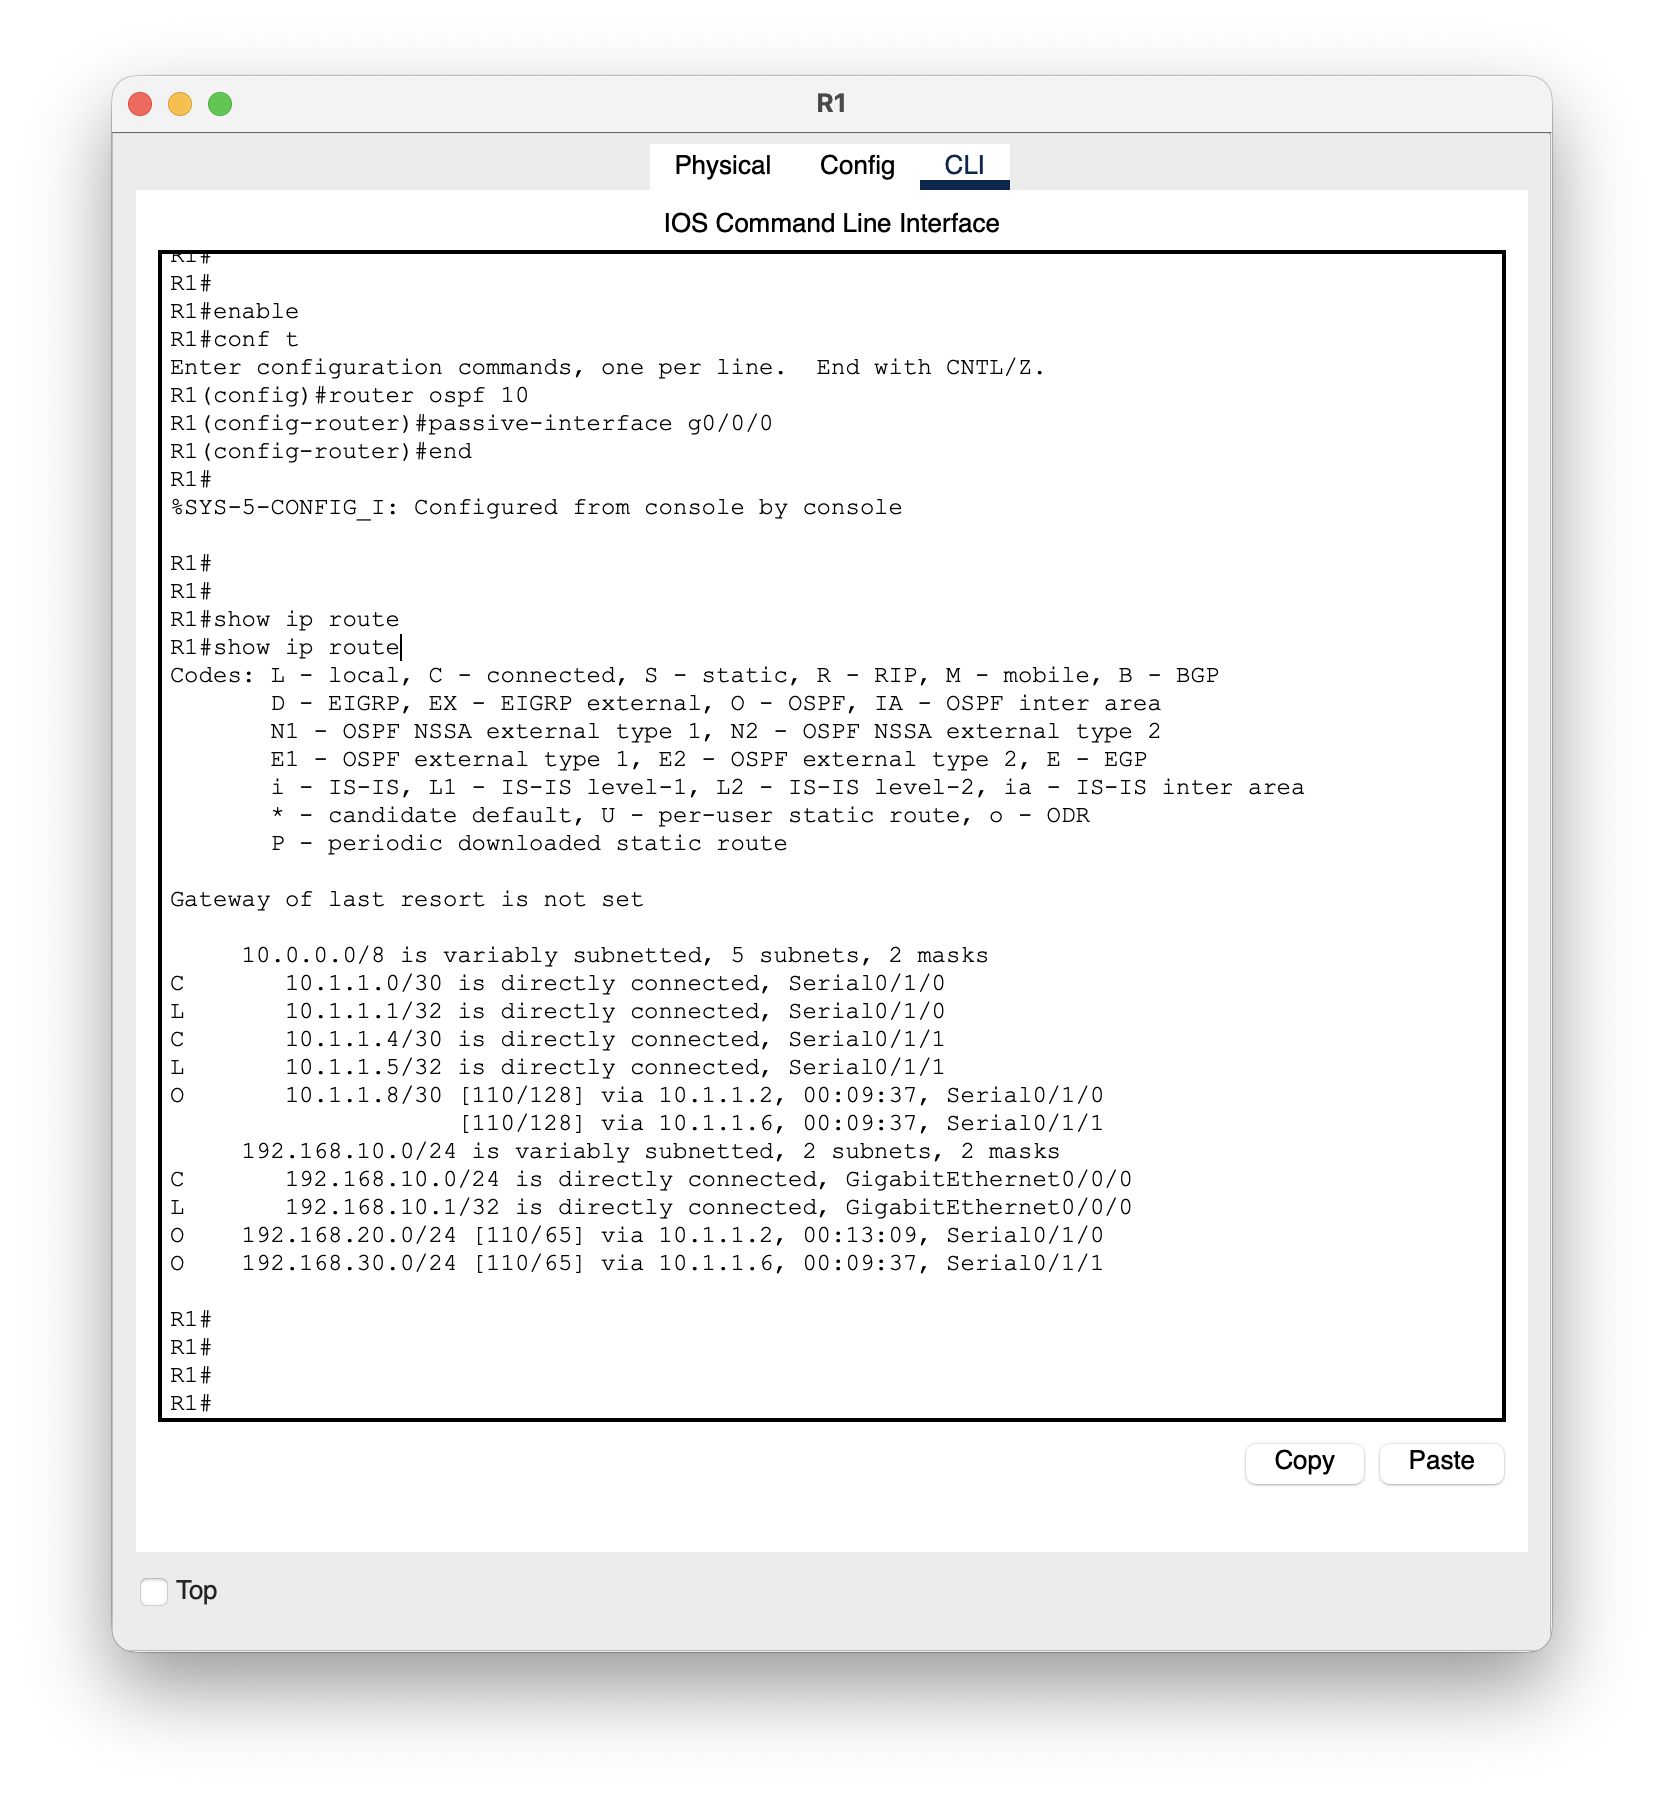
\includegraphics[width=0.95\textwidth]{showiprouteR1.png}
    \caption{Tabla de enrutamiento de R1 mediante \texttt{show ip route}.}
    \label{fig:route-r1}
\end{figure}

\subsubsection{R2}

\begin{figure}[H]
    \centering
    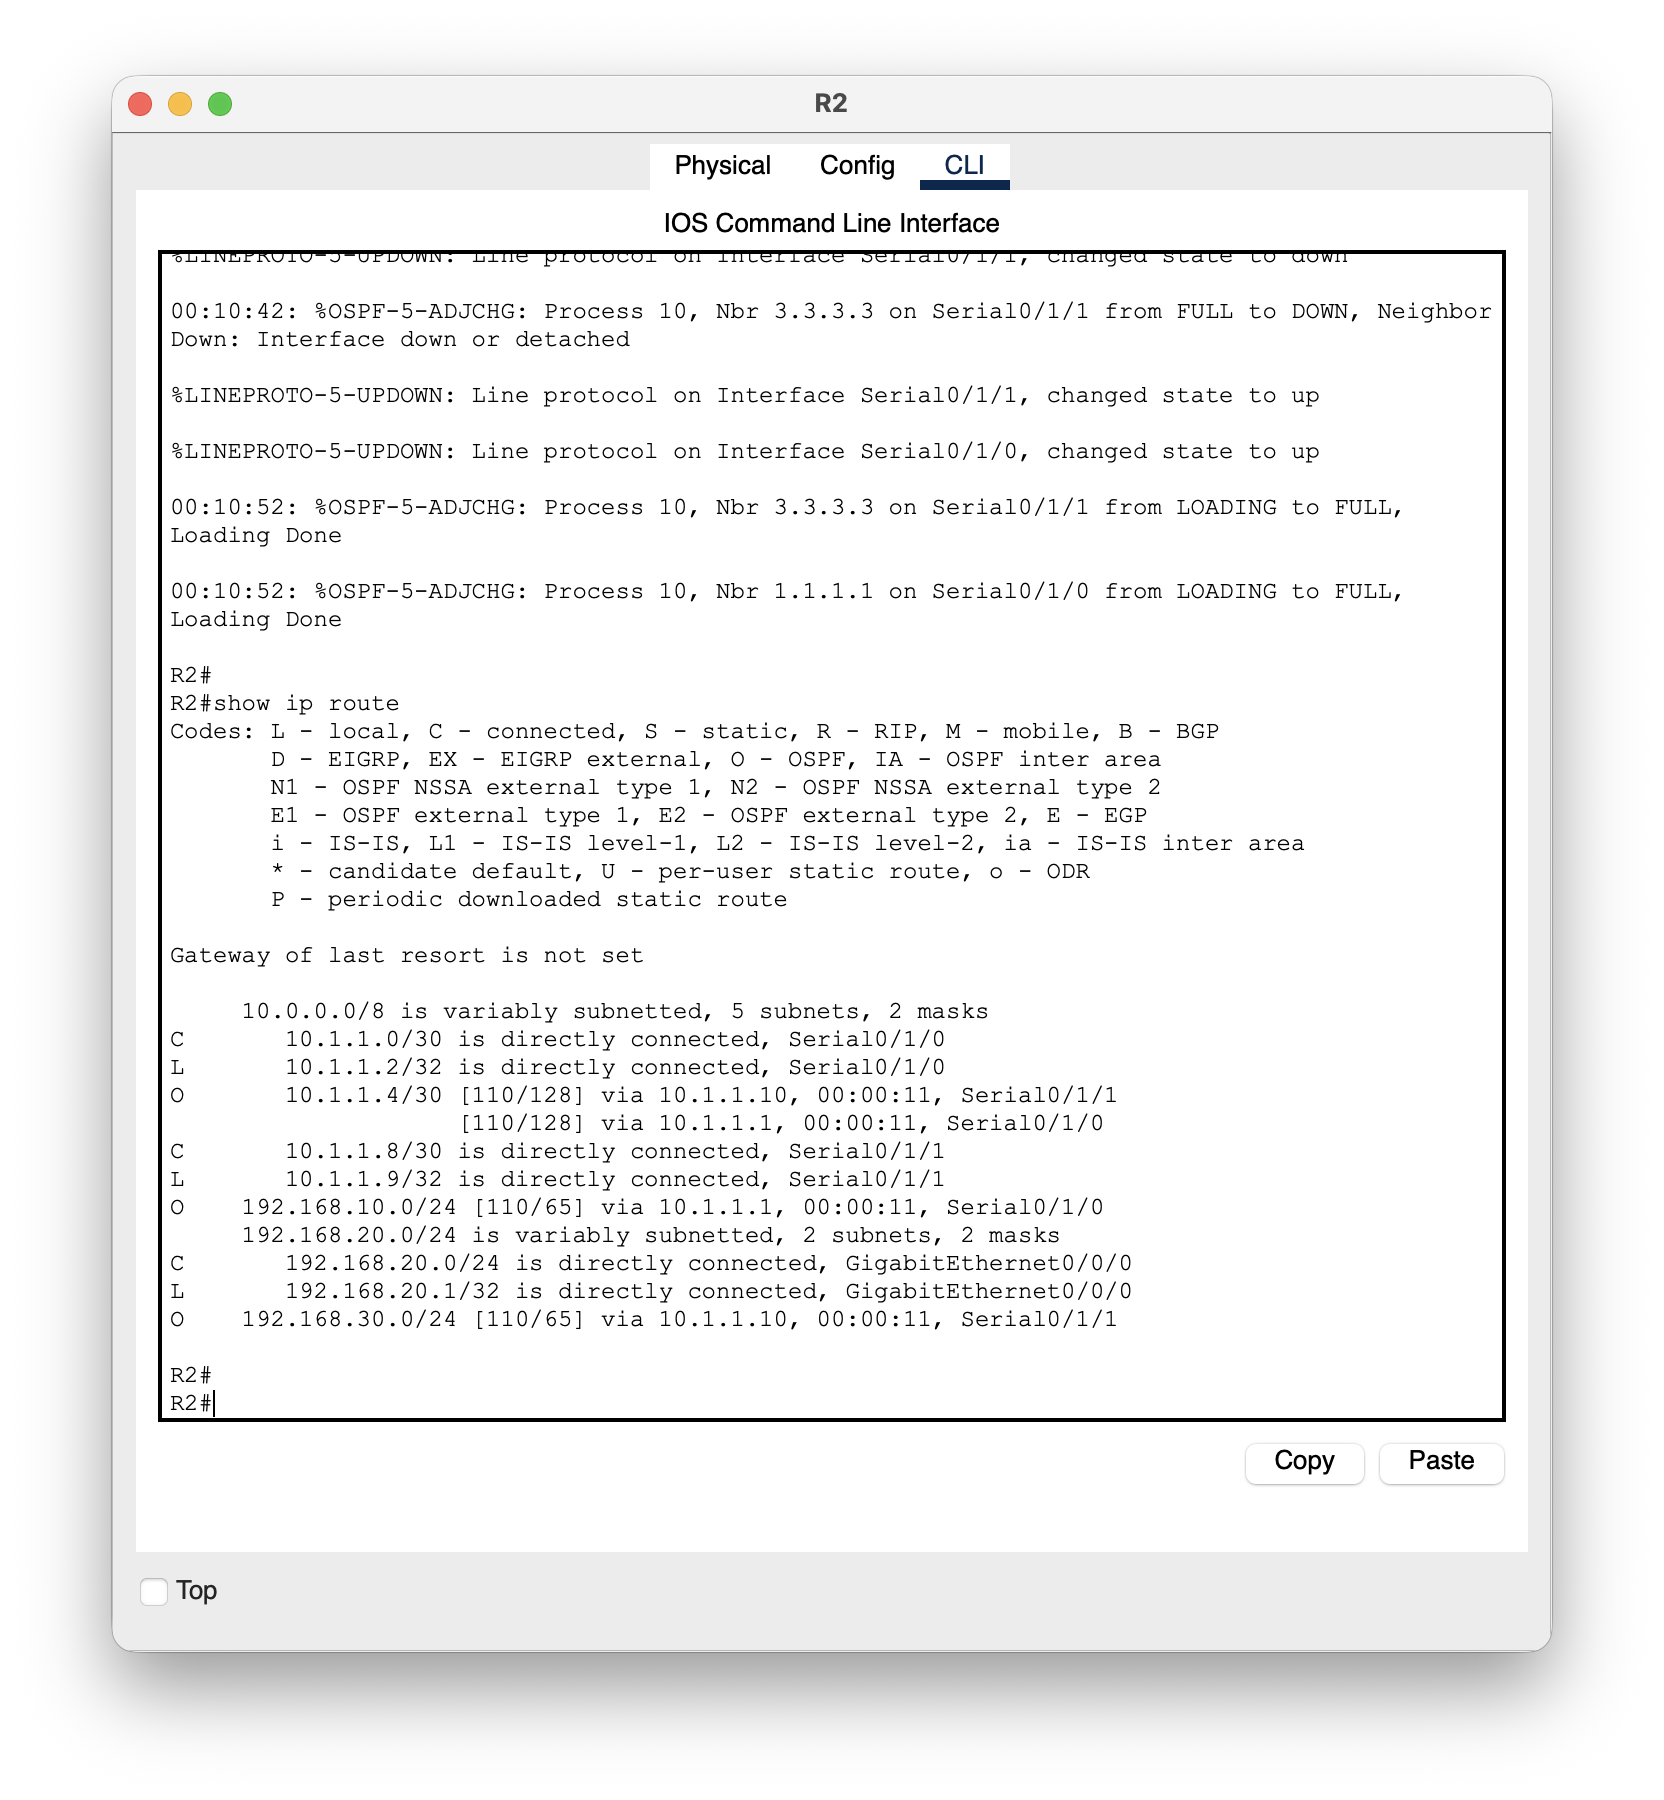
\includegraphics[width=0.95\textwidth]{showiprouteR2.png}
    \caption{Tabla de enrutamiento de R2 mediante \texttt{show ip route}.}
    \label{fig:route-r2}
\end{figure}

\subsubsection{R3}

\begin{figure}[H]
    \centering
    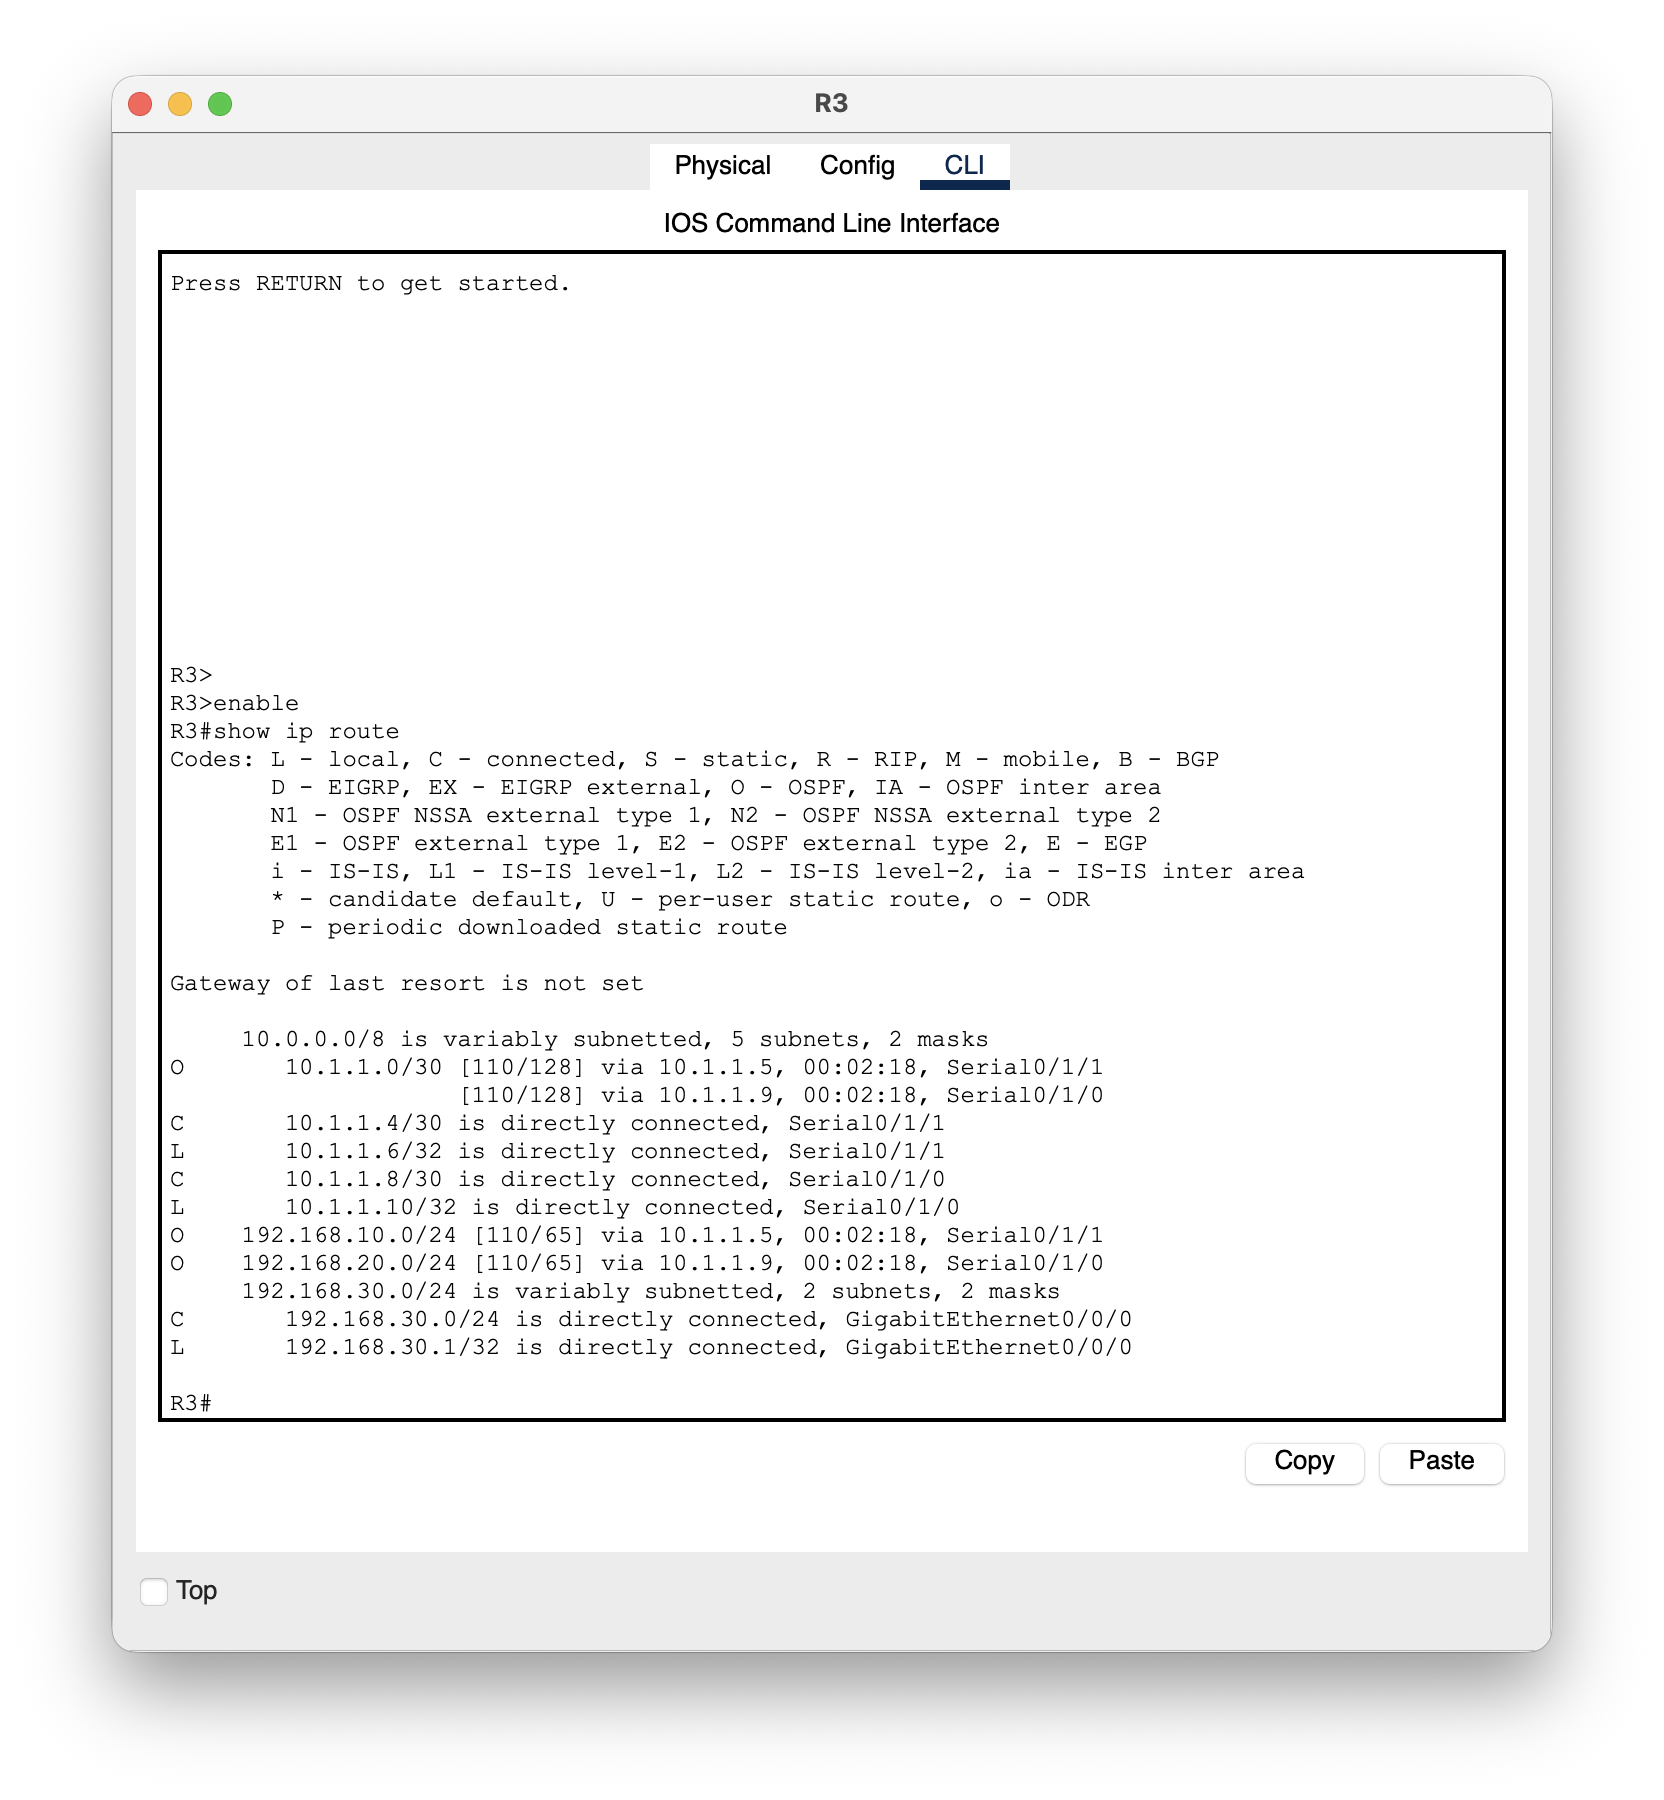
\includegraphics[width=0.95\textwidth]{showiprouteR3.png}
    \caption{Tabla de enrutamiento de R3 mediante \texttt{show ip route}.}
    \label{fig:route-r3}
\end{figure}

\subsection{Verificación de vecinos OSPF}

Para comprobar que los routers establecieron correctamente sus
adyacencias se utilizó:

\begin{lstlisting}[style=cisco]
show ip ospf neighbor
\end{lstlisting}

Este comando muestra los routers vecinos descubiertos mediante OSPF,
incluyendo su Router ID y el estado de la relación.

\subsubsection{R1}

\begin{figure}[H]
    \centering
    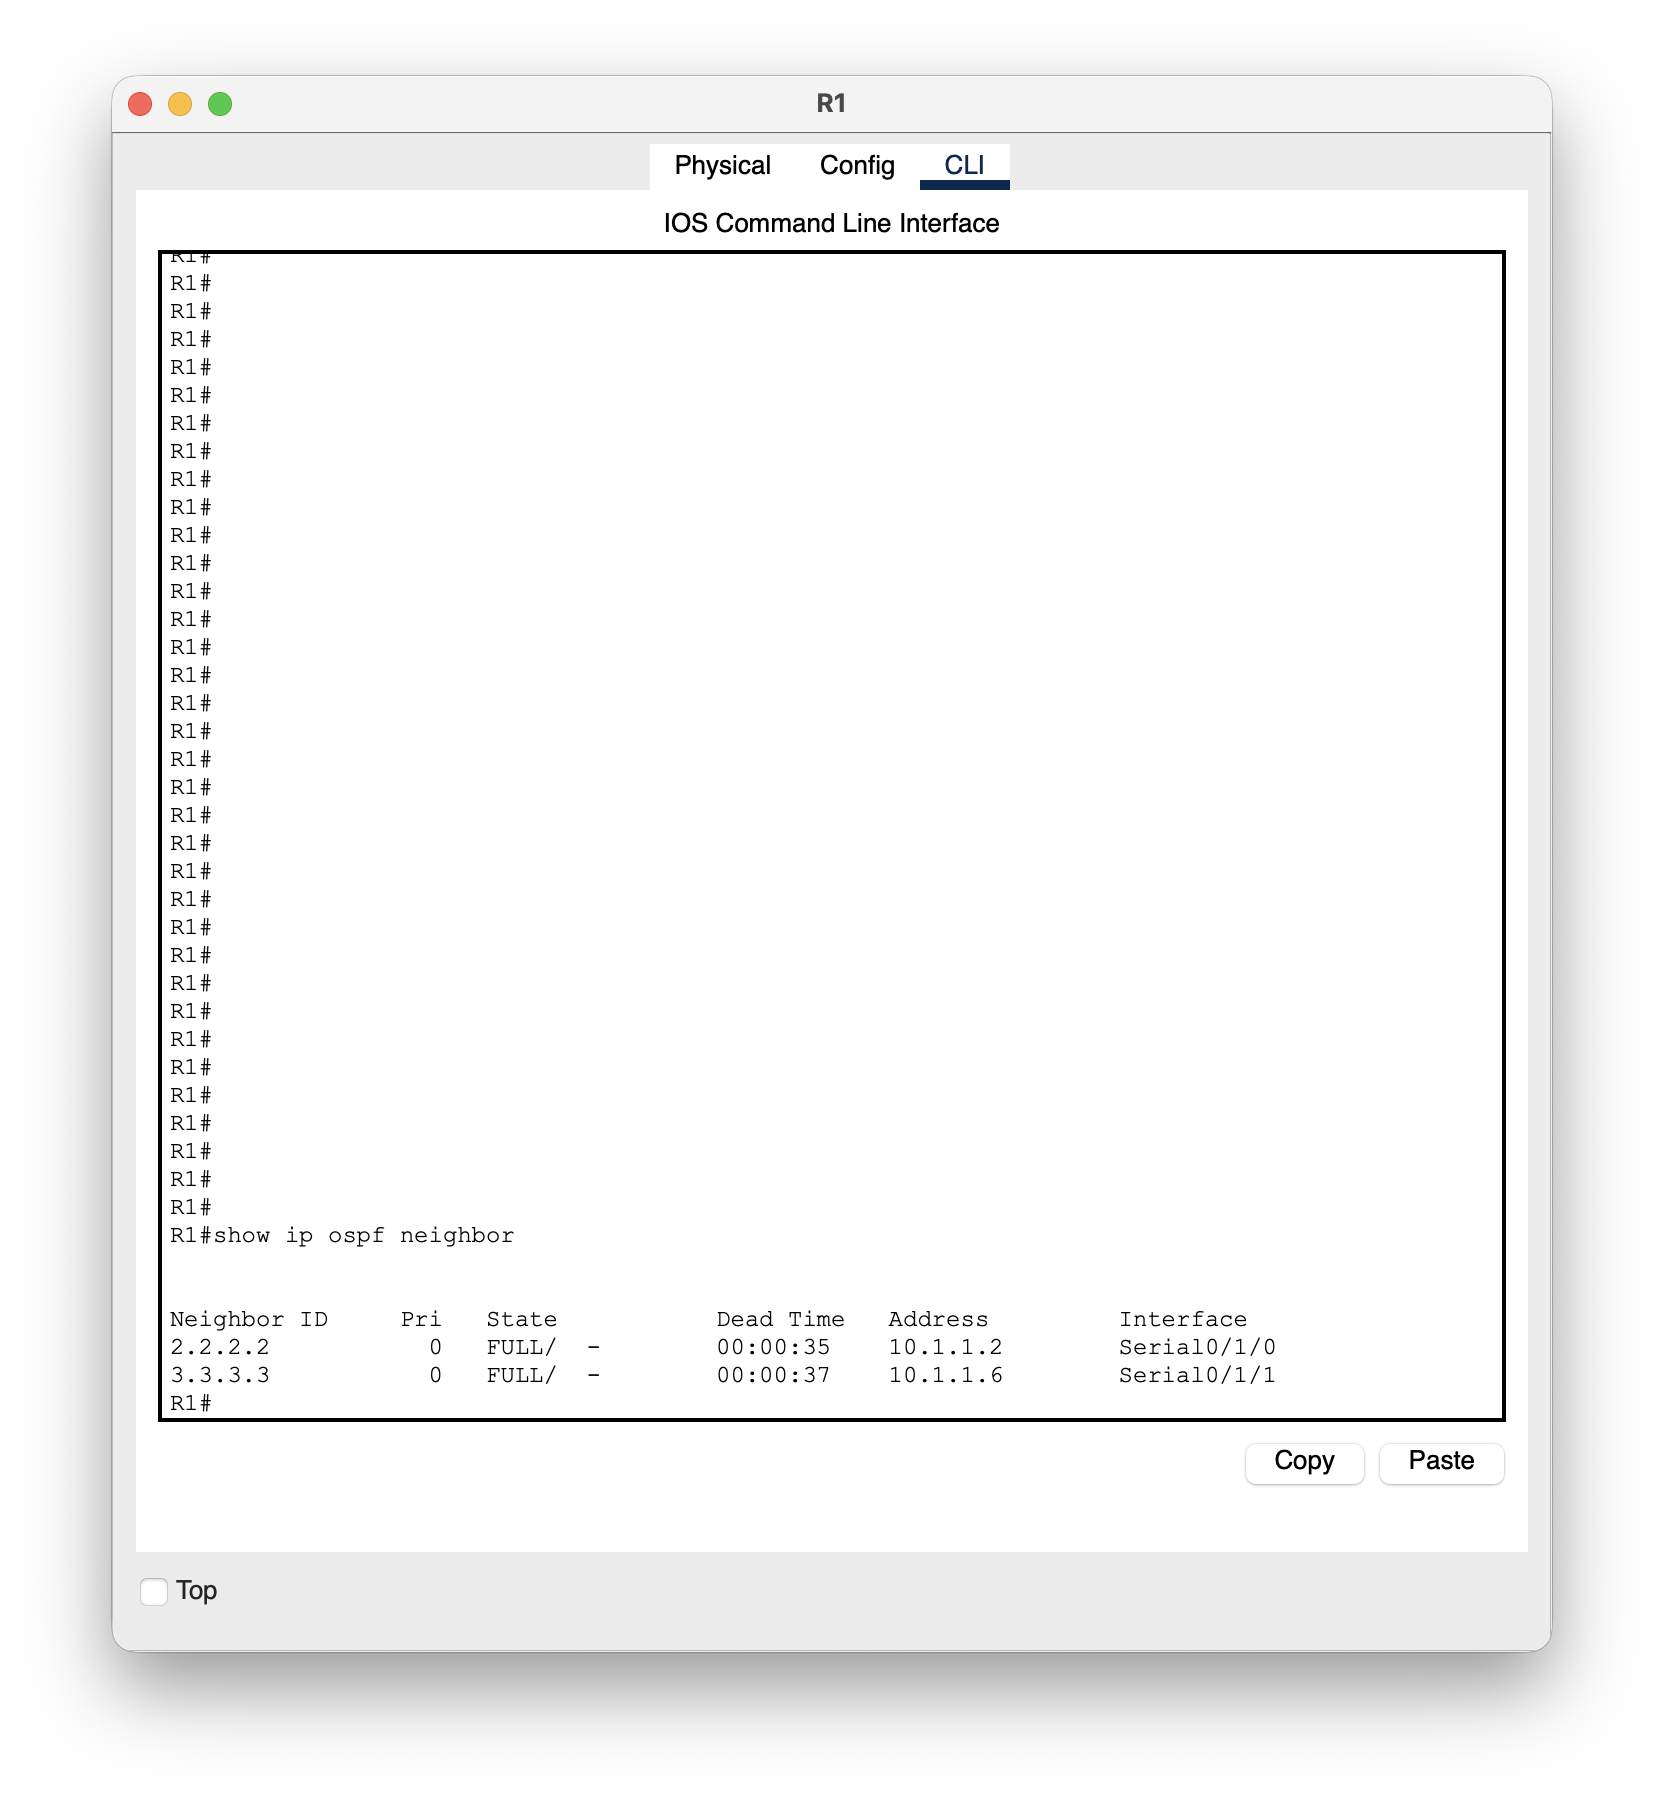
\includegraphics[width=0.95\textwidth]{neighbourR1.png}
    \caption{Vecinos OSPF de R1.}
    \label{fig:neighbor-r1}
\end{figure}

\subsubsection{R2}

\begin{figure}[H]
    \centering
    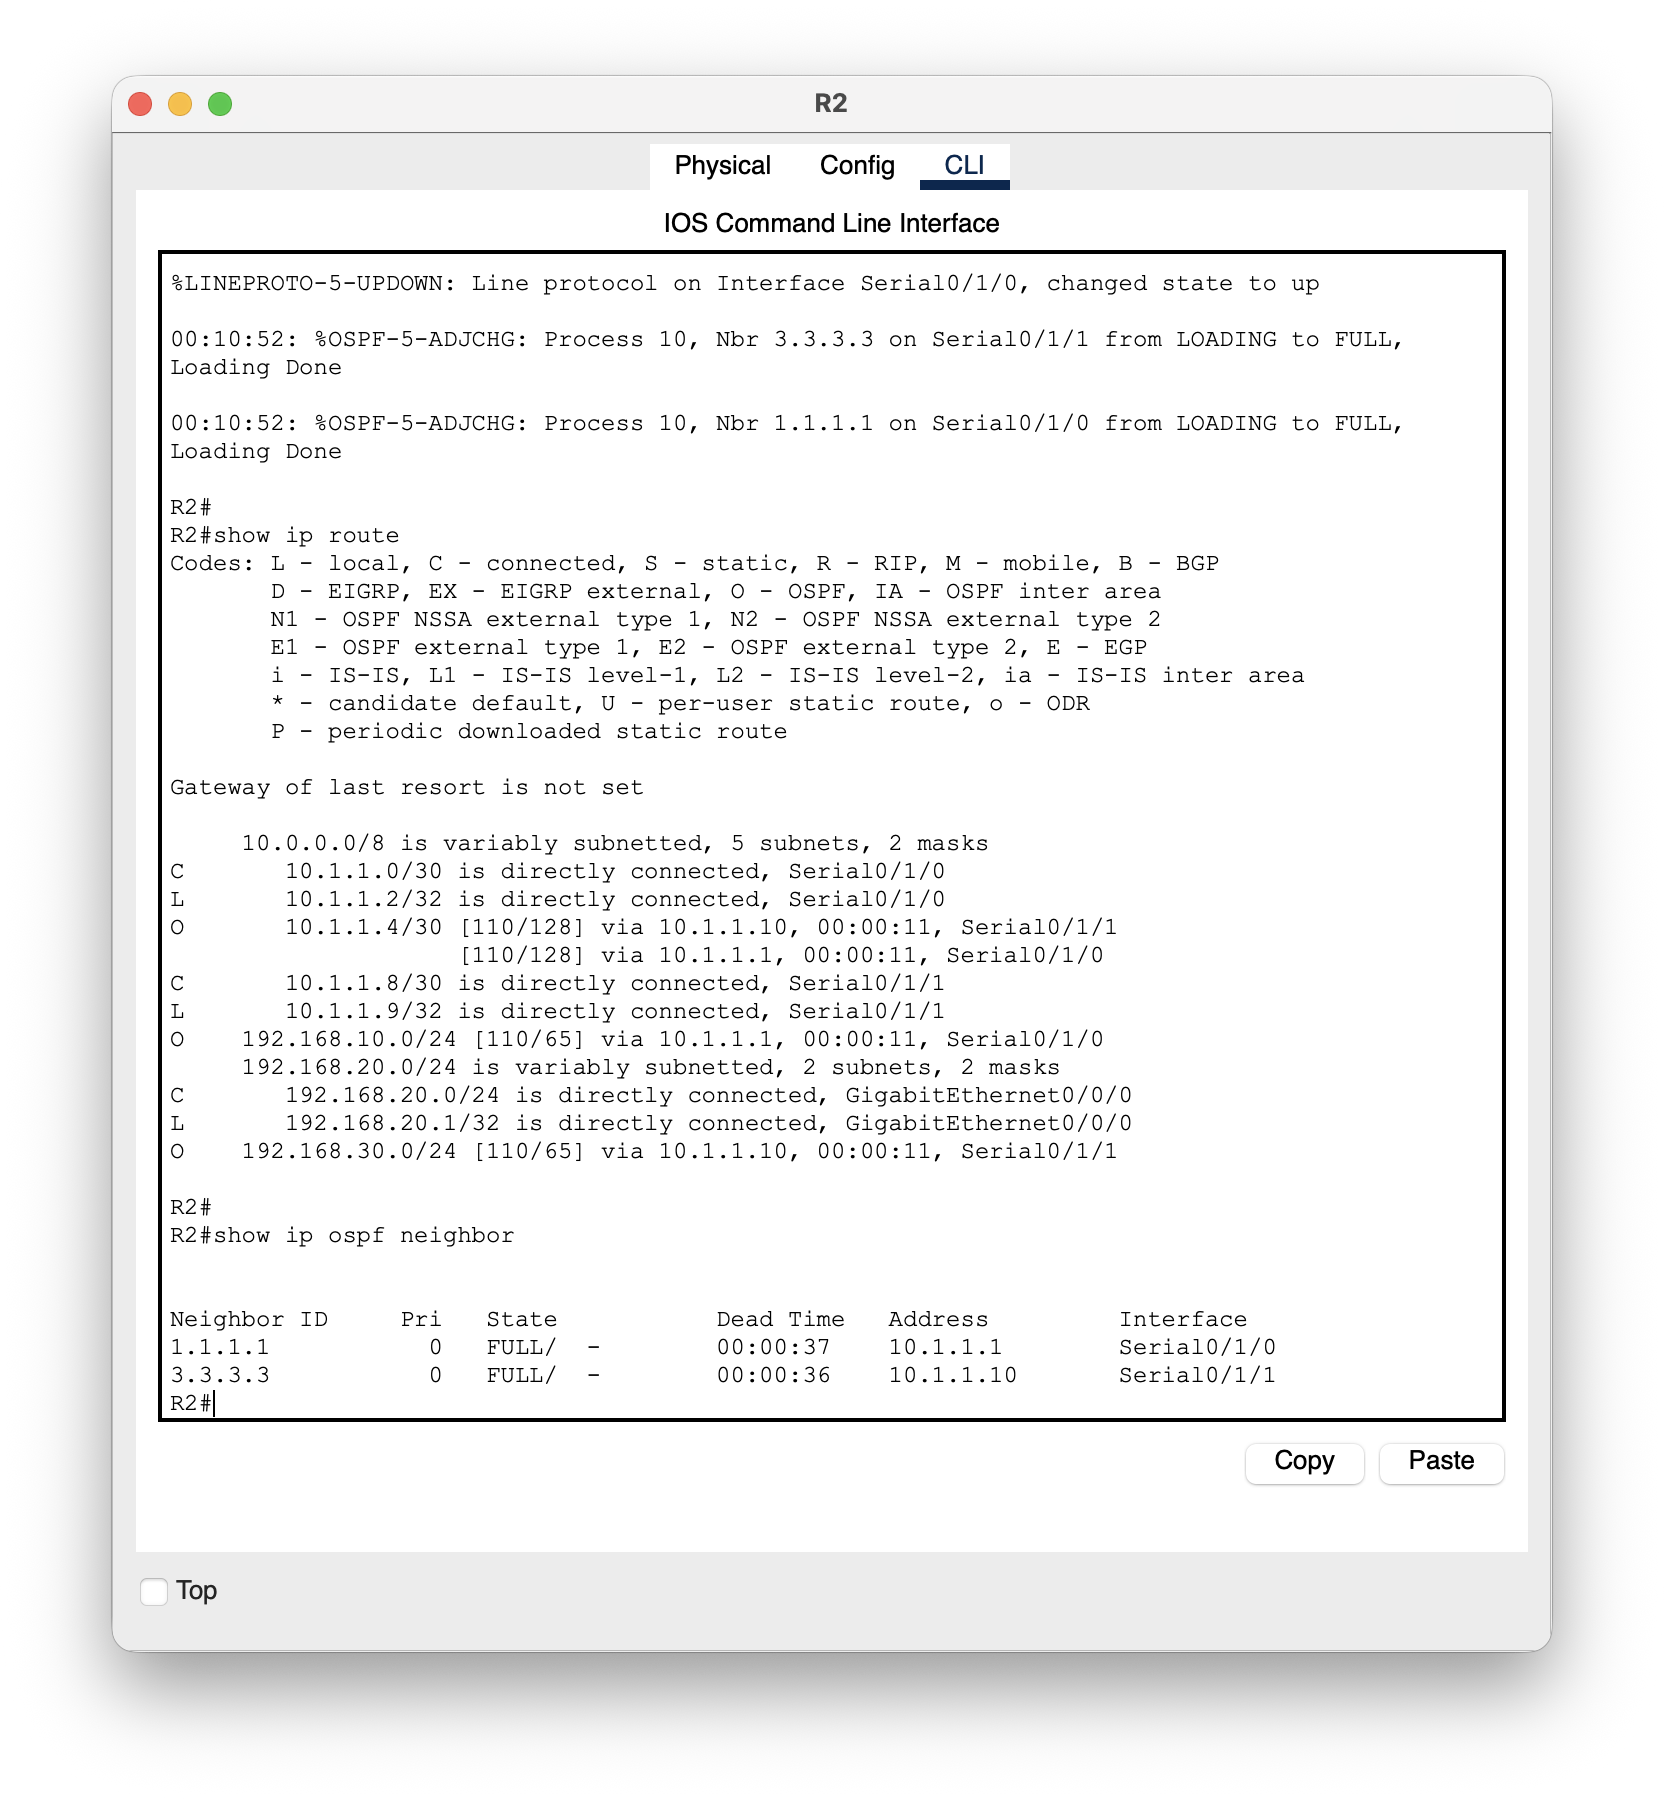
\includegraphics[width=0.95\textwidth]{neighbourR2.png}
    \caption{Vecinos OSPF de R2.}
    \label{fig:neighbor-r2}
\end{figure}

\subsubsection{R3}

\begin{figure}[H]
    \centering
    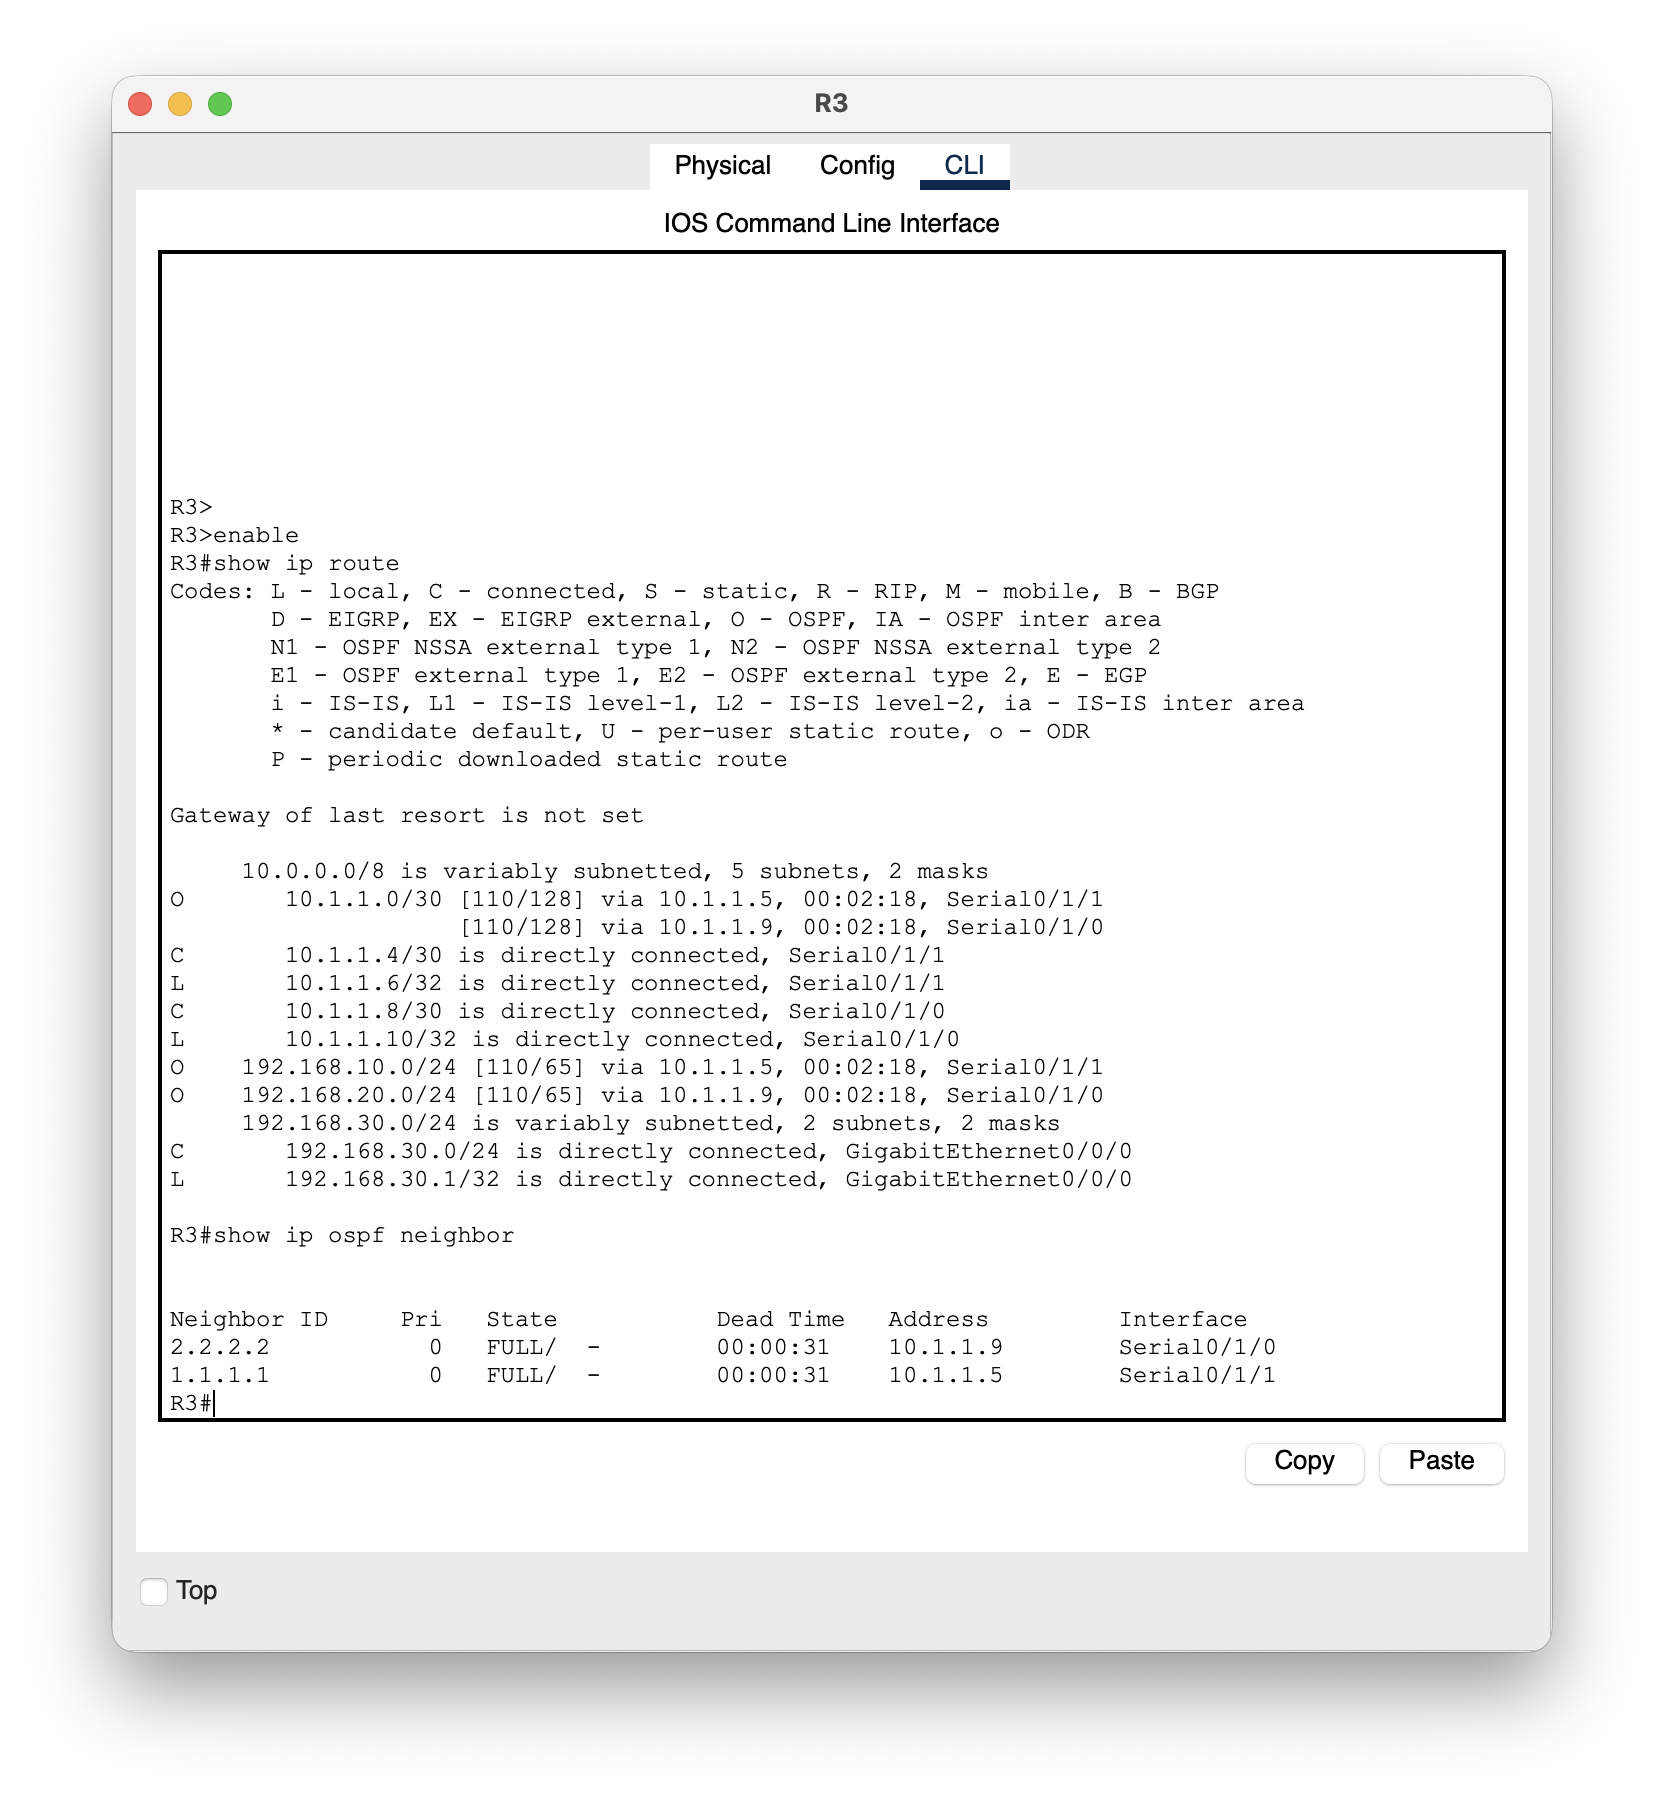
\includegraphics[width=0.95\textwidth]{neighbourR3.png}
    \caption{Vecinos OSPF de R3.}
    \label{fig:neighbor-r3}
\end{figure}

El estado \texttt{FULL} en las relaciones entre los routers indica
que las adyacencias OSPF fueron establecidas correctamente.

% --------------------------------------------------
% RESULTADOS
% --------------------------------------------------
\section{Resultados}

Como resultado de la configuración, los tres routers participaron en
un único dominio OSPF correspondiente al área 0. Cada router recibió
un identificador explícito y estableció relaciones de vecindad con los
routers conectados directamente mediante los enlaces seriales.

La configuración también permitió comprobar tres métodos diferentes
para activar OSPF:

\begin{table}[H]
\centering
\caption{Métodos de configuración de OSPF utilizados}
\begin{tabular}{lll}
\toprule
\textbf{Router} & \textbf{Método} & \textbf{Ejemplo} \\
\midrule
R1 & Red + wildcard & \texttt{network 192.168.10.0 0.0.0.255} \\
R2 & IP + wildcard 0.0.0.0 &
\texttt{network 192.168.20.1 0.0.0.0} \\
R3 & Configuración por interfaz &
\texttt{ip ospf 10 area 0} \\
\bottomrule
\end{tabular}
\end{table}

Las tablas de enrutamiento permitieron verificar que los routers
aprendieron las redes remotas mediante OSPF. Asimismo, las tablas de
vecinos confirmaron la formación de las adyacencias entre los tres
routers.

La siguiente captura muestra la comprobación final de los resultados
de la práctica.

\begin{figure}[H]
    \centering
    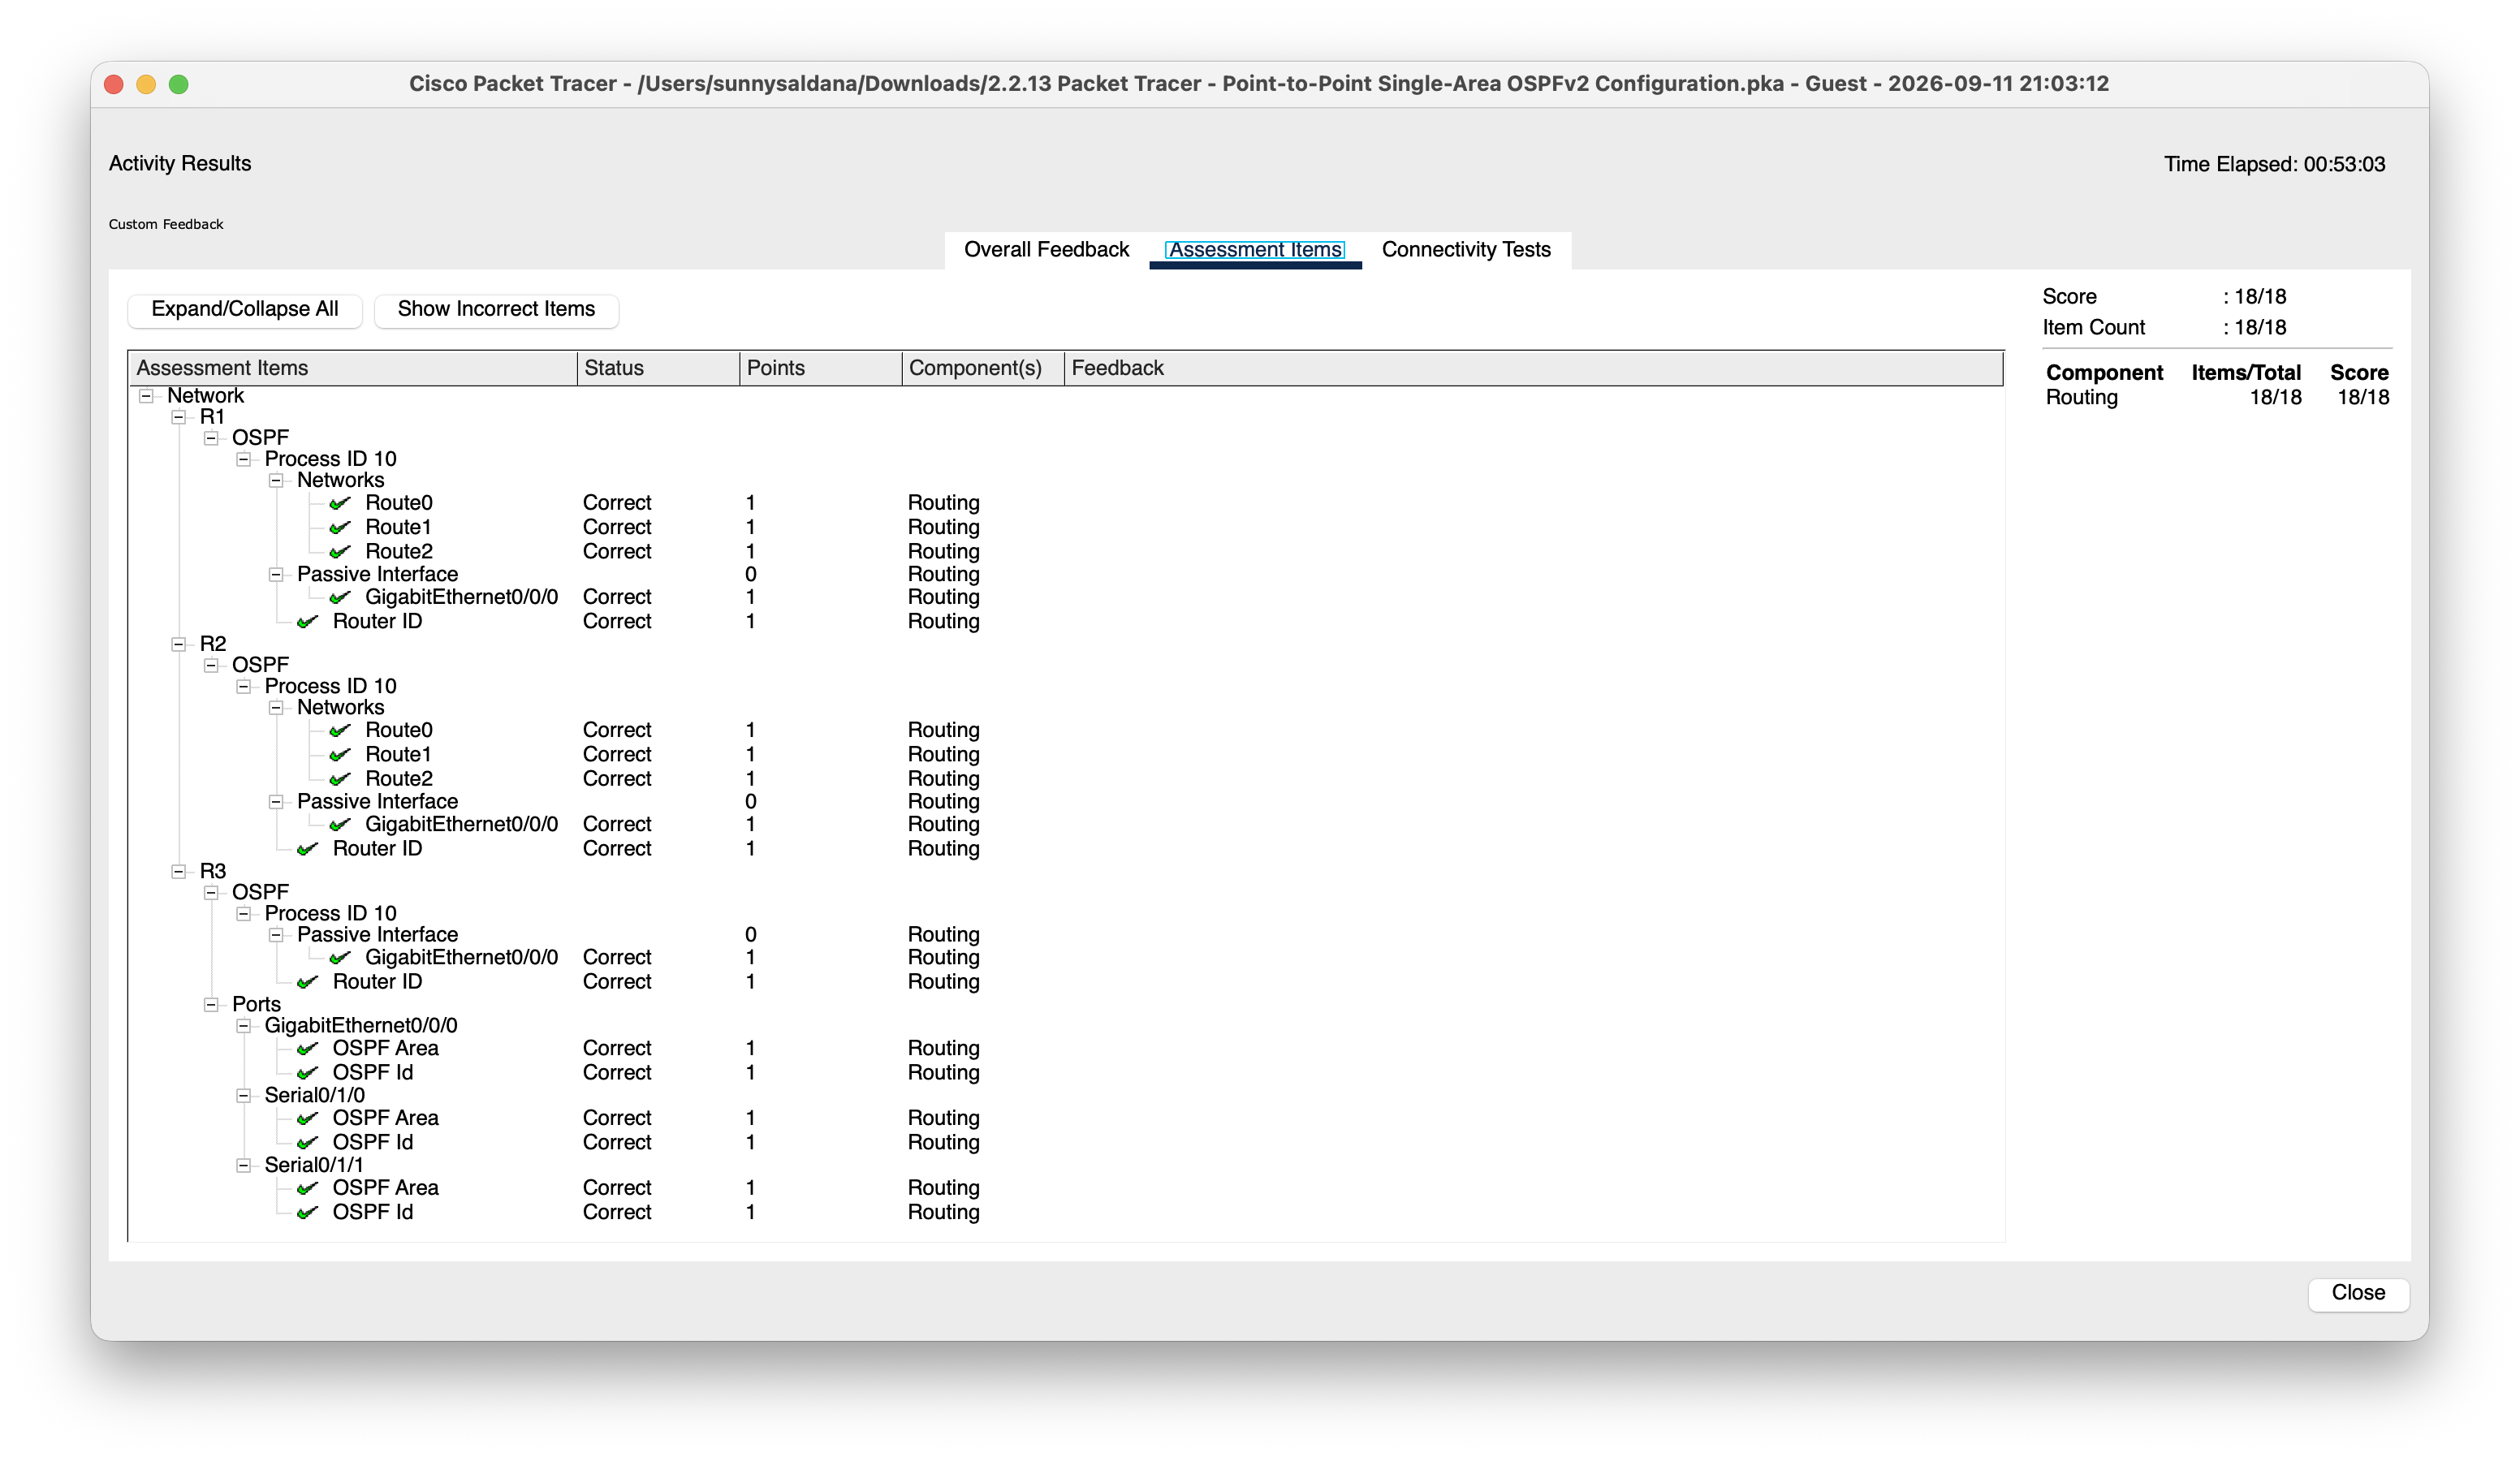
\includegraphics[width=0.95\textwidth]{checkResults.png}
    \caption{Comprobación final de los resultados de la práctica.}
    \label{fig:check-results}
\end{figure}

% --------------------------------------------------
% RESPUESTAS
% --------------------------------------------------
\section{Respuestas a las preguntas de la práctica}

\subsection{¿Cuántas instrucciones se requieren para configurar OSPF
para enrutar todas las redes conectadas a R1?}

Se requieren \textbf{tres instrucciones \texttt{network}}, debido a que
R1 tiene tres redes directamente conectadas:

\begin{itemize}
    \item 192.168.10.0/24
    \item 10.1.1.0/30
    \item 10.1.1.4/30
\end{itemize}

\subsection{La LAN conectada a R1 tiene una máscara /24. ¿Cuál es su
equivalente decimal?}

La máscara /24 corresponde a:

\[
\boxed{255.255.255.0}
\]

\subsection{¿Cuál es el resultado de restar la máscara de subred de
255.255.255.255?}

Para una máscara /24:

\[
255.255.255.255 - 255.255.255.0
=
\boxed{0.0.0.255}
\]

Por lo tanto, \texttt{0.0.0.255} es la máscara comodín correspondiente
a una red /24.

\subsection{¿Cuál es el equivalente decimal de una máscara /30?}

La máscara /30 corresponde a:

\[
\boxed{255.255.255.252}
\]

\subsection{¿Cuál es el resultado de restar la máscara /30 de
255.255.255.255?}

\[
255.255.255.255 - 255.255.255.252
=
\boxed{0.0.0.3}
\]

Por lo tanto, \texttt{0.0.0.3} es la máscara comodín correspondiente a
una red /30.

\subsection{¿Qué interfaces de R3 deben configurarse con OSPF?}

Las tres interfaces de R3 deben configurarse con OSPF:

\begin{itemize}
    \item G0/0/0
    \item S0/1/0
    \item S0/1/1
\end{itemize}

La interfaz G0/0/0 conecta R3 con su red LAN, mientras que las
interfaces seriales permiten establecer comunicación con los otros
routers.

\subsection{¿Qué interfaces son LAN en R1, R2 y R3?}

Las interfaces LAN son:

\begin{itemize}
    \item R1: G0/0/0
    \item R2: G0/0/0
    \item R3: G0/0/0
\end{itemize}

Estas interfaces fueron configuradas como pasivas para evitar el
intercambio innecesario de mensajes de protocolo OSPF hacia las redes
LAN.

% --------------------------------------------------
% CONCLUSIONES
% --------------------------------------------------
\section{Conclusiones}

Durante esta práctica se configuró y verificó el protocolo de
enrutamiento dinámico OSPF en una topología compuesta por tres
routers. El ejercicio permitió comprender que OSPF puede activarse
mediante diferentes mecanismos dependiendo de la configuración que se
desee realizar.

En R1 se utilizaron direcciones de red junto con máscaras comodín para
seleccionar las interfaces participantes. En R2 se utilizaron las
direcciones IP específicas de las interfaces acompañadas de la
máscara \texttt{0.0.0.0}, mientras que en R3 se configuró OSPF
directamente sobre cada interfaz mediante \texttt{ip ospf}.

También se comprendió la importancia de las máscaras comodín dentro de
las instrucciones \texttt{network}. Estas se obtienen invirtiendo los
bits de la máscara de subred y permiten determinar qué direcciones IP
deben coincidir con cada instrucción.

Finalmente, la configuración de interfaces pasivas permitió distinguir
entre las interfaces que necesitan intercambiar información OSPF y
aquellas en las que únicamente se encuentra una red final. La
verificación mediante \texttt{show ip route} y
\texttt{show ip ospf neighbor} permitió confirmar tanto el aprendizaje
de rutas como el establecimiento de las adyacencias entre los routers.

Con esto se logró implementar un esquema de enrutamiento dinámico en
el que las tres redes LAN pueden comunicarse entre sí sin necesidad de
configurar manualmente cada ruta remota.

\end{document}